\documentclass[10pt,openright,twoside,french]{book}

\input philippe2013
\input philippe2013_cours
\input philippe2013_sections
\input philippe2013_chapitre

\setcounter{chapter}{11}
\begin{document}

\renewcommand\PartProgramme{Fonctions}
\chapter[Fonctions polynôme de degré 2, fonctions homographiques]{Fonctions polynôme de degré 2\\ Fonctions homographiques}\label{ch_degre2_homograhique}

\section{Fonction polynôme de degré 2}

\begin{Defi}
    On appelle \iptb{fonction polynôme de degré 2}\index{fonction!polynôme} toute fonction $f$ définie pour tout $x \in \R$ par : \[f(x) = ax^2 + bx + c\] où $a$, $b$ et $c$ sont des nombres réels tels que $a\neq 0$.
\end{Defi}

\begin{Rmq}
	On dira parfois simplement polynôme de degré $2$ ou encore \ipt{trinôme}.
\end{Rmq}


\begin{Exemple}
	\begin{enumerate}
		\item $3x^2+4x + 8$ : $a = 3$, $b = 4$, $c = 1$.
		\item $-x^2+2x - 3$ : $a = -1$, $b = 2$, $c = -3$.
		\item $-2x^2 + 6$ : $a = -2$, $b = 0$, $c = 6$.
		\item $-2x+5 -9x^2$ : $a = -9$, $b = -2$, $c = 5$.
	\end{enumerate}
\end{Exemple}

\begin{Defi}
	On appelle \ipt{parabole} la courbe représentative d'une fonction polynôme de degré dans un repère orthogonal. Le \ipt{sommet} de la parabole est le point le plus haut ou le plus bas de la parabole.
\end{Defi}

\begin{Prop}
	Soit $f$ une fonction polynôme de degré $2$. Il existe 2 réels $\alpha$ et $\beta$ tels que, pour tout $x \in \R$, \[f(x) = a(x - \alpha)^2 + \beta.\]
\end{Prop}

\begin{Prop}
	Soit $f$ une fonction polynôme de degré $2$ écrite sous la forme $a(x - \alpha) + \beta$.\par
	Alors $\beta = f(\alpha)$ et $\beta$ est le maximum ou le minimum de la fonction $f$, atteint pour $x = \alpha$.\par
	On en déduit que le sommet de la parabole représentant $f$ a pour coordonnées $(\alpha \pv \beta)$.
\end{Prop}

\begin{Demo}
	$f(x) = a(x - \alpha)^2 + \beta$ donc $f(\alpha) = a(\alpha - \alpha)^2 + \beta = \beta.$\smallskip

	\begin{description}
		\item[$a > 0$ :] Pour tout $x \in \R$,
		$(x-\alpha)^2 \geq 0 \Leftrightarrow a(x-\alpha)^2 \geq 0 \Leftrightarrow a(x-\alpha)^2 + \beta \geq \beta \Leftrightarrow f(x) \geq \beta$\par
		donc $\beta$ est le minimum.\smallskip
		
		\item[$a < 0$ :] Pour tout $x \in \R$,
		$(x-\alpha)^2 \geq 0 \Leftrightarrow a(x-\alpha)^2 \leq 0 \Leftrightarrow a(x-\alpha)^2 + \beta \leq \beta \Leftrightarrow f(x) \leq \beta$\par
		donc $\beta$ est le maximum.
	\end{description}
\end{Demo}

On en déduit alors les situations suivantes :\medskip

\begin{minipage}{0.45\linewidth}
	\begin{center}
		$a > 0$\medskip
		
	\begin{tikzpicture}
		\tkzTabInit[nocadre,espcl=2]{$x$/1,Variations \\ de $f$/1.5}{$-\infty$,$\alpha$,$+\infty$}
		\tkzTabVar{+/,-/$\beta$,+/}
	\end{tikzpicture}

	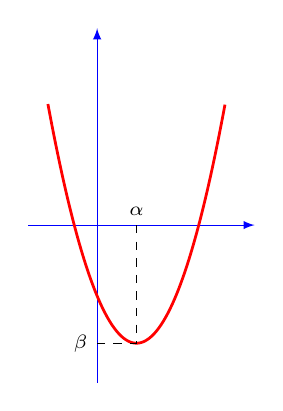
\begin{tikzpicture}[>=latex,scale=0.5]
		\draw[->,blue] (-1.75,0)--(4,0);
		\draw[->,blue] (0,-4)--(0,5);
		\draw[color=red,line width=1pt] plot[domain=-1.25:3.25,samples=200] (\x,{1.2*(\x - 1)^2 - 3});
		\draw[dashed] (1,0) node[above] {\scriptsize $\alpha$}|-(0,-3) node[left] {\scriptsize $\beta$};
	\end{tikzpicture}
    
	\end{center}
\end{minipage}



	



\end{document}
